

\chapter{Introduction}\label{C:intro}
\section{Introduction}
Modern enterprises need to respond effectively and quickly to opportunities in today's competitive and global markets. 
To accommodate business agility, companies are supposed to start with use existing applications instead of
developing them from scratch. 
A contemporary approach for addressing these critical issues is embodied by (Web) services that can be 
easily assembled to form a collection of autonomous and loosely coupled business processes \cite{Papazoglou}.

The arising of web service developments and standards in support of automated business integration has 
driven major technological advances in the integration software space, most notably, 
the Service Oriented Architecture (SOA) \cite{Dan:2008}. In an SOA, software resources are packaged as 
web services, which are well defined, self-contained modules that provide standard business functionality
and are independent of the state or context of other services \cite{Ran}.

A web service is a software system allowing to expose web services via the Internet. The 
SOA promotes the composition of coarse-grained web services to build more complex
web applications using standards such as WS-BPEL \cite{std/ws-bpel2}. Because of the convenience, 
low cost and capacity \cite{Aboolian} to be composed into high-level business processes, web service technology is becoming increasingly popular.


With the ever increasing number of functional similar web services being available on the the Internet, the Web Service Providers (WSPs) are trying to improve the quality of service (QoS) to become competitive in the market.  
QoS, also known as non-functional requirements to  web service, is the degree to which a web service meets specified requirements or user needs \cite{4061431}, such as response time, security and availability. 
Among numerous QoS measurements, service response time is a critical factor for many real-time services, e.g. traffic service or finance service. 

Service response time has two components: transmission time (variable with message size) and network latency \cite{Johansson}. 
Study \cite{916684} shows that network latency is a significant component of web service response delay.
Ignoring network latency will underestimate response time by more than 80 percent \cite{Sun}, since network latency is related to network topology as well as physical distance \cite{distanceMetrics}. 
To reduce the network latency, large web service providers like Google, Facebook or Microsoft have their own high-bandwidth data centers. The majority of WSPs
can not afford to build a data center, therefore they rent servers provided by Web Server Hosting Providers (WSHPs). WSPs need to allocate their services wisely so that the overall network latency is minimized. 
According to a popular web traffic analyzing company Alexa, 96\% of top one million web services were hosted
in heterogeneous server clusters or co-location centers \cite{He} that were widely distributed across different geographic regions. 
Hence, it is necessary to provide an effective web services allocation guide to WSPs so that they can be benefited.


The Web service location allocation problem is very challenging because it is a combinatorial optimization problem. A combinatorial optimization has 
a non-continuous and rugged search space, which makes it difficult to search for the optimal solutions. Furthermore, Web service location allocation problem is
essential a multi-objective optimization problem \cite{Multiobjective} for which there are two conflicting objectives, to minimize latency and total cost.
Previous researches \cite{Aboolian, Sun} use integer programming and greedy algorithm to solve this problem. However, these approaches are either easy to be stuck at 
local optima or performs poorly when problem size increases.

Multi-objective Evolutionary Optimization Algorithm (MOEA) methodologies are ideal for solving multi-objective optimization problems \cite{key:article}, 
since MOEAs work with a population of solutions.
With an emphasis on moving towards the true Pareto-optimal region, a MOEA algorithm can be used to find multiple Pareto-optimal solutions in 
one single simulation run \cite{OptimizationElectrical}. 
Specifically, \cite{godinez2010,hassan2005} discover that Particle Swarm Optimization (PSO)-based multi-objective optimization algorithms has the same or better effectiveness as 
the Genetic Algorithm (GA)-based multi-objective optimization algorithms but with significantly better computational efficiency (less function evaluations). 
Therefore, PSO-based algorithms are chosen to solve the problem.


\section{Objectives}
The overall goal is to develop a new PSO-based approach to the Web service location allocation problem by considering two potentially 
conflicting objectives - minimizing cost and minimizing network latency. 

To accomplish this goal, we design three objectives:
\begin{enumerate}
 \item Develop an aggregating approach using PSO which combines two objectives into a single fitness function and investigate whether the aggregating
	approach can do a good job for balancing the two conflicting objectives.
 \item Develop a Pareto front approach using multi-objective nondominated-sorting PSO (NSPSO). It is the first time that NSPSO is 
	used to solve Web service location allocation problem, and we investigate whether the Pareto front approach outperforms the aggregating approach.
 \item Develop a new multi-objective PSO approach by considering better diversity and performance when problem size increases. We investigate whether
	this approach can produce better performance than the aggregating and Pareto front approaches.
\end{enumerate}



\section{Major Contributions}
 The project has three contributions. 
 \begin{enumerate}
 \item This project shows that an aggregating approach converge well and be able to achieve the optimal solution in small problems.
 \item This project shows that a NSPSO Pareto front approach achieve better performance than aggregating approach. It can provide a set of solutions that are distributed more diversely
 than the aggregating approach.
  \item This project presents a new multi-objective PSO-based approach with two major improvements. 
      Firstly, We develop a rounding function mechanism which transforms a continuous algorithm to a binary algorithm. 
      The dynamic rounding function provides better results with good diversity. 
      Secondly, we develop an adaptive threshold mechanism which embodies the idea of transfer learning. 
      Similar to dynamic rounding function, it also provides the ability to solve binary problem and promising results.
      Another desired feature of dynamic and adaptive rounding functions is that they perform well regardless of the sizes of problems.
 \end{enumerate}

\section{Organization}
The report is organized as follows. 
Chapter \ref{C:background} provides background information. 
Chapter \ref{C:single} presents a detailed Web service location allocation problem description and model formulation. 
It also presents a BPSO with an aggregating approach. 
Chapter \ref{C:multi} presents a NSPSO-based approach. 
Chapter \ref{C:bmopsocd} presents a new binary multi-objective PSO with crowding distance. 
Chapter \ref{C:clu} provides a discussion of the conclusion and some remaining future work.

\chapter{Background}
\label{C:background}
\section{Web Service Location Allocation}
Service-oriented computing (SOC) provides a new paradigm for building distributed computing applications over the Internet. It gradually changes
the way of software design, distribute and consume. In SOC, web services are the building blocks to support effective, low-cost development of applications
in different environments \cite{bougue}.
SOC depends on service-oriented architecture (SOA) to organize applications and infrastructures into a set of interacting web services. The recent development of web service provides a common framework that allows data to be shared and reused across applications, enterprises and community boundaries. That is, web services become on-line resources. 

% Similar to traditional industry, Web service providers and
% customers can be benefited from an appropriate allocation of web services. 
% From WSPs' perspective, it minimizes the number of deployed servers. 
% From customers' perspective, it improves the QoS. 

% Similar to Web Service location allocation, Cloud computing resource management has encountered the similar problem\cite{5598294}. 
% The fundamental \textbf{objectives} of these two problems 
% include optimizing allocation price, and QoS such as availability, security and response time \cite{7083783}.

In order to provide good Quality of Service (QoS), the fundamental objectives are optimizing the properties of QoS such as
availability, security and response time. Availability \cite{Kritikos} represents the probability that a service in available, a large value denotes the service is always ready to use while a small value denotes the service is unstable. Security \cite{Anisetti} is a measurement of web service of providing access control, encrypting messages. Security is now becoming more important because web service invocation occurs over the public Internet.
Response time is a major measurement of service performance while low latency values indicate low response time. Latency
is the round trip time between sending a request and receiving the response.  Latency is now the main impediment to improving performance \cite{Flach}. Since network latency is related to network topology
as well as physical distance \cite{distanceMetrics}, it is hard to reduce latency by analysing the underlying network topology.
A straightforward way to reduce latency is that treat network as a black box and allocate services according to round trip experiments \cite{cha2008design}. 
This is the main reason that WSPs need to choose service locations carefully.

Some service users may have specific requirements such as fast response time and strong availability. These constraints
 must be considered before launching web services. 
 WSPs may also have constraints such as an overall cost constraint. In different locations, 
 WSHPs might charge different prices. There are two ways to reduce the overall cost, deploying less
 services or deploying services in locations with low price.
 In addition, 
 a common constraint is the service number constraint which ensures every service is deployed at least to one location.

In this project, we consider minimizing latency and overall cost as the objectives because response time is one of the most important service performance measurements and the overall cost is the major concern of WSPs. For the sake of simplicity, we
only consider a service number constraint.

We introduce some terminologies used in a Web service location allocation context.
To solve the Web service location allocation problem, 
some basic information must be provided by \emph{Web Service Providers (WSPs)}. A WSP must provide a list 
of \emph{user centers} and a list of \emph{candidate locations}. A user center indicates a center city of an \emph{user concentrated area}. 
This step can be achieved by analyzing web service requests data from existing web services or conducting a market survey. 
A candidate location is the geometric location that is suitable to 
deploy web services (e.g. existing \emph{Web Server Hosting Providers (WSHPs)}). 
The selection of a candidate location is based on other criteria such as facilities or rental fees of servers. 
User centers and candidate locations are not necessarily overlapped.
A WSP also need to provide \emph{service invocation frequency}, \emph{network latency} and \emph{web service fixed deployment cost} at each candidate location. 
\emph{Service invocation frequency} denotes the number of invocations from an user center
to a web service within a period of time; \emph{network latency} denotes the average latency between user centers and candidate locations over a period of time;
\emph{web service fixed deployment cost} denotes the rental of a server in each candidate location.

In summary, the list below shows some critical information that should be provided by the WSPs.

\begin{enumerate}
	\itemsep0em
	\item A list of user centers
	\item A list of candidate locations
	\item Service invocation frequencies from user centers to web services
	\item Average network latency from user centers to candidate locations
	\item Web service fixed deployment cost at each candidate location
\end{enumerate}

It is worth noting that the data in the above list are changing over time and some of the changes are critical,
for example, the invocation frequency from a user center $U$ to a web service $W$ drops rapidly. 
It indicates that the web service $W$ was once popular in $U$ became unfrequented.
At this point, existing web services need to be re-allocated in order to adapt the market. Other scenarios such as,
the network latencies vary in different time periods within a day. Existing web services do not need to re-allocated because 
the average network latency remains stable.


\begin{figure}[!htb]
   \centering
   \begin{subfigure}{0.4\textwidth}
       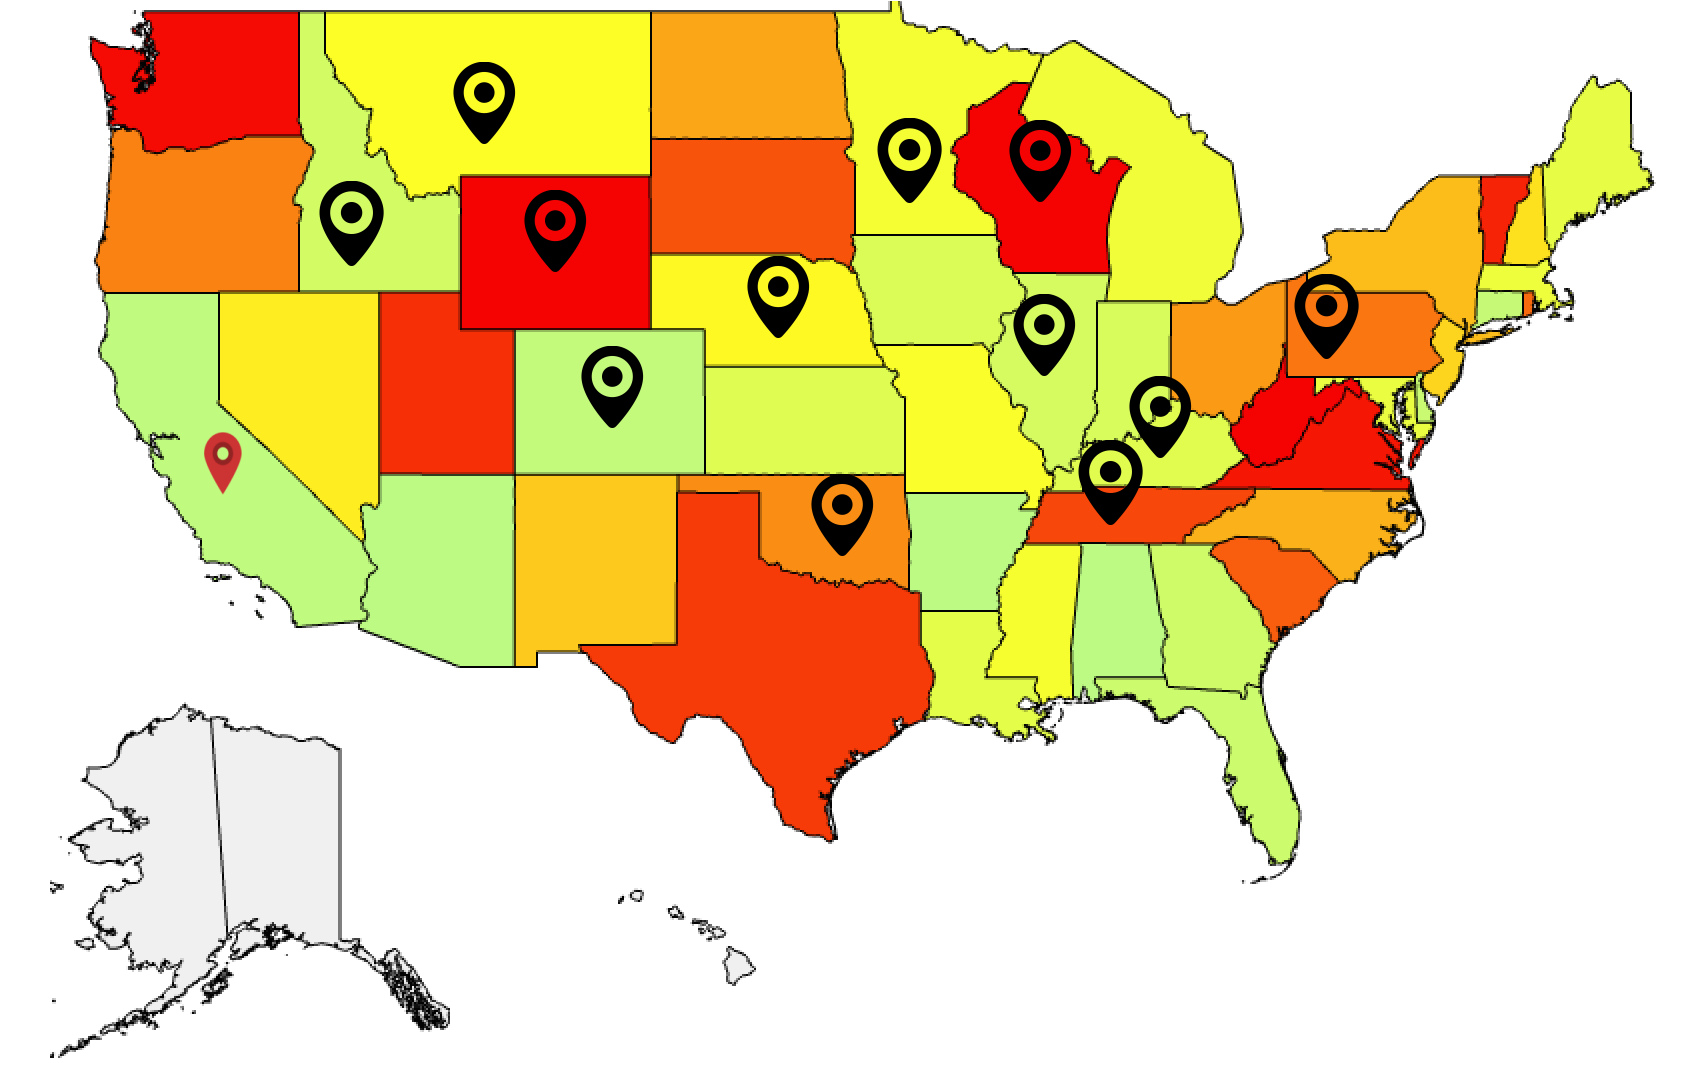
\includegraphics[width=\textwidth]{pics/web1.png}
	   \caption{web service $A$}
   \end{subfigure}
   \begin{subfigure}{0.4\textwidth}
       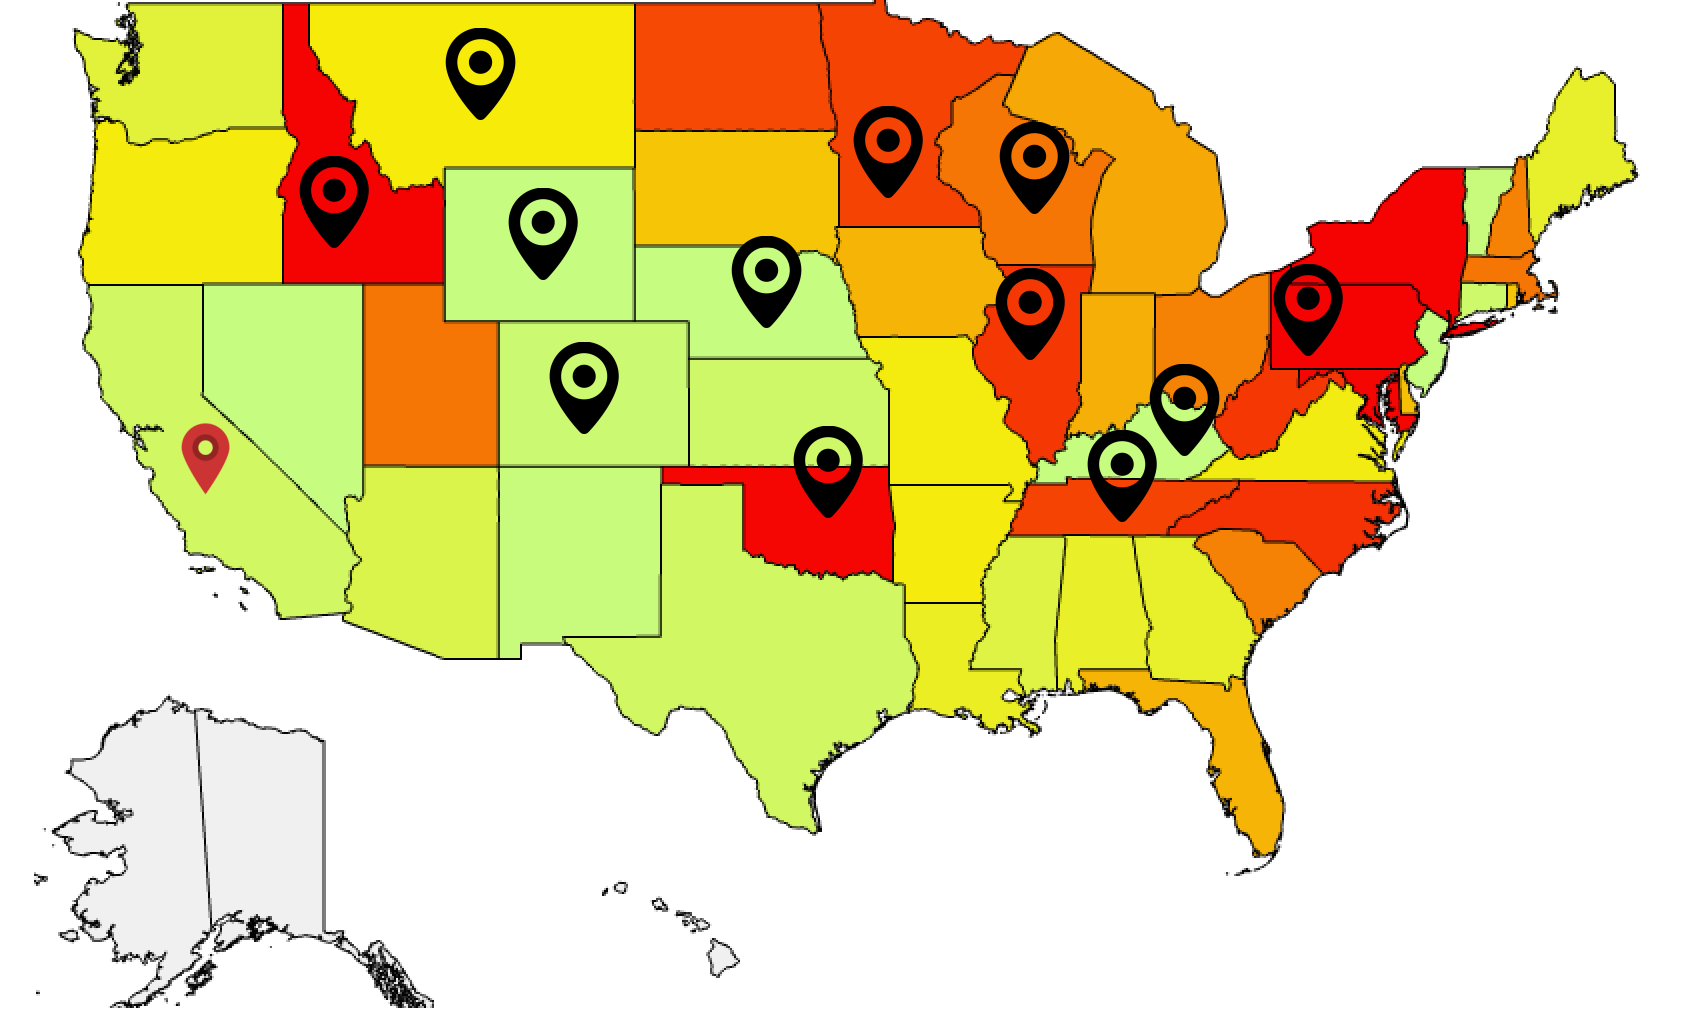
\includegraphics[width=\textwidth]{pics/web2.png}
	   \caption{web service $B$}
   \end{subfigure}
   \caption{User distribution of two web services}
   \label{fig:users}
\end{figure}


We illustrate these terminologies with a simple example (Figure \ref{fig:users}). 
A Web service provider has $N$ web services initially deployed in San Francisco, California (red pin on Figure \ref{fig:users}). During the next a few months, the WSP constantly received complaints
from all over the country about the high response time of the services. The WSP seeks some ways to improve the quality. They found a straightforward
way to re-allocate the web services. Therefore, they conducted a statistical analysis over the 
raw data that are collected from web services. Based on the data analysis, the WSP found each web service has its own \emph{user concentrated area} (each state) . 
For example, Figure \ref{fig:users} shows the popularity of web services $A$ and $B$ across the country.
Red denotes high popularity while green denotes low. In each state, a city is selected as the \emph{user center} (e.g. the capital city).
The black pins denote the \emph{candidate locations} which are also cities select from states. 
As we can see the user distributions are quite distinct for $A$ and $B$. Now the WSP would choose locations for these web services.
The WSP soon realized the problem is too complex to use any analytical methods for the following reasons:
\begin{enumerate}
 \item Large number of web services
 \item Large number of candidate locations and user centers
 \item Trade-off between minimizing cost and minimizing network latency
 \item Constraints (e.g. minimal web service number requirement)
\end{enumerate}




\section{Evolutionary Computation}
Evolutionary Computation is a subfield of Artificial Intelligence. It is very well-known for its effective global search ability. These algorithms are 
inspired by biological mechanisms of evolution, social interactions and swarm intelligence. 
There are several distinguished characteristics of EC algorithms such
as the use of a population and the ability of avoiding local optima. 
A common process of EC algorithms is as follows. Initially, the population are randomly generated in the search space. During the evolution process, the population
moves according to a predefined fitness function. At the end of the evolution, the individual with the best fitness value is selected as the output.

The origins of evolutionary computation can be traced back to 1950s \cite{back1997evolutionary}. Since 1970s, the output of EC research has grown exponentially. 
The majority of current implementations of EC algorithms descend from three major approaches: \emph{genetic algorithms}, \emph{evolutionary programming}
and \emph{evolution strategies}.

GA \cite{holland1962outline} was introduced by Holland. There is a large number of applications uses GA \cite{de1992genetic, de1993genetic}.
Evolutionary programming, introduced by Fogel \cite{fogel1962autonmous}, was originally designed to generate artificial intelligence. 
Evolutionary strategies as developed by Rechenberg \cite{rechenberg1971} and Schwefel \cite{Schwefel1975}, were initially designed with the goal of solving difficult discrete
and continuous, mainly experimental, parameter optimization problems \cite{klock}. 

In the next a few sections, we introduce the background knowledge of each
algorithm we will use in this project.


\subsection{Particle Swarm Optimization (PSO)}
PSO was proposed by Kennedy and Eberhart in 1995 \cite{488968}. PSO is a population based meta-heuristic algorithm 
inspired by the social behavior of birds and fishes. In PSO, each individual is called a particle which flying
around the search space. The underlying phenomenon of PSO is optimized by social interaction 
where particles sharing information to direct their movement.


PSO is based on the principle that each solution can be represented as a 
particle. At initial state, each particle has a random initial position in the 
search space which is represented by a vector $x_i = (x_{i1}, x_{i2}, \dots, x_{iD})$, where \emph{D} is the dimensionality of the search space.
Each particle has a velocity, represented as $v_i = (v_{i1}, v_{i2}, \dots, v_{iD})$ which is limited by a 
predefined maximum velocity, $v_{max}$ and  $v_{id}$ $\in$ $[-v_{max}, v_{max}]$. 
During the search process, each particle maintains a record of previous best performance, called $pbest$. The best position of its neighbors 
is also recorded, which is $gbest$. The position and velocity of each particle are 
updated according to the following equations:

\begin{equation}
	x^{t+1}_{id} = x^{t}_{id} + v^{t+1}_{id}
\end{equation}
\begin{equation}
	v^{t+1}_{id} = w * v^{t}_{id} + c_1 * r_{1i} * (p_{id} - x^t_{id}) + c_2 * r_{2i} * (p_{pg} - x^i_{id})
\end{equation}

In the two equations, $t$ shows the $t^{th}$ iteration. \emph{d} $\in$ \emph{D} 
shows the $d^{th}$ dimension. \emph{w} is the inertia weight used to balance the local search and 
global search abilities of PSO. $c_1$ and $c_2$ are acceleration constants. 
$r_{1i}$ and $r_{2i}$ are random constants uniformly distributed in $[0, 1]$. $p_{id}$ and $p_{gd}$ denote the values of $pbest$ and $gbest$ in $d^{th}$ dimension.

\subsection{Binary PSO}
PSO was originally developed to address continuous optimization problems. 
Therefore, the representation for both position and velocity of a particle in 
PSO is a vector of real numbers. However, this representation is not suitable 
for many discrete optimization problems. To address the discrete problem, in 1997 
Kennedy and Eberhart developed a binary 
particle swarm optimization (BPSO) \cite{637339}.
In BPSO, the position of each particle is a vector of binary numbers, which are 
restricted to 1 or 0.  The velocity in BPSO represents the probability of the 
corresponding position taking value of 1. A sigmoid function is used to transform a velocity
between 0 and 1. The following equation is 
used to update the position of each particle:

\begin{equation}
\label{eq:updatePosition}
		x_{id} = 
		\begin{cases}
			1 & \quad \text{if } rand() < s(v_{id})\\
			0 & \quad \text{otherwise} \\
		\end{cases}
\end{equation}
\begin{equation}
\label{eq:updateVelocity}
	s(v_{id}) = \frac{1}{1 + e^{-v_{id}}}
\end{equation}
The $rand()$ is a random number selected from a uniform distribution in $(0, 1)$.

\subsection{Multi-Objective Evolutionary Optimization Algorithm}
Multi-objective Evolutionary Optimization Algorithm (MOEA) was initially designed in the mid-1980s. Since then, people find MOEAs both efficient and
effective because MOEAs deal simultaneously with a set of possible solutions which allow us to find multiple non-dominated solutions in 
a single run. Additionally, MOEAs are less suffering from the shape or continuity of the Pareto front (e.g. they can deal with discontinuous and concave
Pareto fronts) \cite{abraham2005evolutionary}. In MOEAs, there are many strategies to deal with multi-objectives. 
The most popular strategy is the linear aggregation approach, 
which aggregates all the objective values into
a single value \cite{coello2006evolutionary}. Nonlinear aggregation approaches were also popular \cite{coello1998two}.
A Pareto front approach was first introduced by Goldberg in his seminal book on GA \cite{goldberg1988genetic}. Goldberg suggested to use nondominated ranking and selection to 
move a population to the Pareto front. This idea currently is the mainstream in MOEA.
\subsection{Non-dominated Sorting Genetic Algorithm II (NSGA-II)}
NSGA-II is a multi-objective algorithm based on genetic algorithm (GA). 
It was proposed by Klyanony et.al \cite{996017} in 2002.
NSGA-II performs well in convergence and permits a remarkable level of flexibility. It has four innovative properties, a fast non-dominated sorting 
procedure, an elitist strategy, a parameterless approach and an efficient constraint-handling method. 

\subsection{Multi-Objective PSO}
Several multi-objective optimization algorithms are based on PSO such as 
Multi-objective PSO (MOPSO) \cite{1304847}, and Non Dominated Sorting PSO (NSPSO) \cite{NSPSO}. 
The performance of different multi-objective algorithms is compared in \cite{1304847} using five test functions. 
These algorithms are NSGA-II \cite{996017}, PAES \cite{knowles2000}, Micro-GA \cite{Micro} and MOPSO. 
The results show that MOPSO is able to generate the best set of non-dominated solutions close to the true Pareto front in all test functions 
except in one function where NSGA-II is superior. Apart from the good optimization ability, another major advantage for PSO-based algorithms is low computational cost. 
They are more effective than other EC algorithms.

Raquel et al. \cite{Raquel} propose a MOPSOCD extended from the MOPSO. 
The mechanism of crowding distance is incorporated into the algorithm on global best selection of an external 
archive of non-dominated solutions. The diversity of non-dominated solutions in the external archive is improved by 
using the crowding distance together with a mutation operator. The performance shows that MOPSOCD is highly 
competitive in generating a well-distributed set of non-dominated solutions. 
%\subsection{Genetic Algorithms (GAs)}
%GA \cite{man1996genetic} is a powerful tool to solve combinatorial optimization problems. It is an iterative procedure based on a constant-size population. In a GA, a population of strings (called chromosomes
%or the genotype of the genome), which are encoded as candidate solutions (called individuals, creatures, or phenotypes) to an optimization problem, evolves towards better solutions. 
%Each genome is associated with a fitness value based on a fitness function that indicates how close it comes to meeting the overall specification, when compared to other genomes in the
%population. The fitness value of an individual is also an indication of its chances of survival and reproduction in the next generation. A typical genetic algorithm requires a genetic
%representation of the solution domain and a fitness function to evaluate the solution domain. Since a chromosome from the population represents a solution, when the algorithm starts, 
%the whole population moves like one group towards an optimal area so the GA searches from a population of solutions rather than a single solution. Integer scalarization technique \cite{Multiobjective} is 
%used to solve multi-objective problems with GA. It predefines a weight for each objective.


%The algorithm starts with a random initialization population. Once the population is sorted based on non-domination sorting, a rank is assigned to each chromosome.
%Then, a parameter called crowding distance is calculated for each individual. The crowding distance is a measure of how close an individual is to its neighbors. A large 
%average crowding distance will result in better diversity in the population. 

%Parents are selected from the population by using tournament selection based on the rank and the crowding distance. An individual is selected in the rank if it is smaller than the other or 
%if the crowding distance is greater than the other. The selected population generates offsprings using crossover and mutation operators. 

%The population with the current population and current offsprings is sorted again based on non-domination and only the best N individuals are selected, where N is the population size.
%The selection is based on rank and the on crowding distance on the last front.

\section{Related work on Service Location Allocation}
\subsection{Traditional Service Location Allocation and Resource Management in Cloud}
\label{sec:drawbacks}
Most of the researchers treat service 
location allocation problem as a single objective problem. \cite{Aboolian, Sun} try to solve the problem by using integer linear programming techniques.
In particular, \cite{Sun} solves this problem by employing greedy and linear relaxation.

Researches on network virtualization \cite{export:149565,export:141114} employs greedy algorithms to allocate virtual machines (VMs) in 
the data center so that the requirements of network bandwidth are met. \cite{6217521} presents
a multi-layer and integrated fashion through a convex integer programming formulation.

The major drawback of greedy algorithm is that it is easy to be stuck at local optima. Integer linear programming
is well-known as not scaling very well. It performs poorly when the number of variables is large.



\subsection{EC Approaches}
Huang \cite{EnhancedGenetic} proposes an enhanced genetic algorithm (GA)-based approach on Web service location allocation. 
He models the problem as a single objective problem with respect to network latency. 
In particular, the position of a web service in a Web service composition workflow is considered in his model.
Kessaci \cite{6557869} proposes MOGA-CB for minimizing cost of VMs instance and response time.
\cite{Phan8} proposes a framework - Green Monster, to dynamically move web services across Internet data centers for reducing 
their carbon footprint while maintaining their performance. Green monster applies a modified version of NSGA-II algorithm \cite{996017}
with an additional local search process.


\section{Summary}

Previous researchers have studied the Web service location allocation problem with single-objective algorithm, linear programming technique and 
greedy algorithm. These approaches have many obvious disadvantages (Section \ref{sec:drawbacks}). 
Web service location allocation problem in nature is a multi-objective problem which should be addressed by multi-objective algorithms. 
From previous study, we found MOEAs are promising. Specifically, among many MOEAs, 
multi-objective particle swarm optimization with crowding distance (MOPSOCD) is a recent development. It outperforms other approaches including NSGA-II, PAES
in various aspects. 
% Therefore, we decide to further improve the MOPSOCD and solve Web service location allocation problem with it.
